\documentclass{mipt-thesis-bs}
% Следующие две строки нужны только для biblatex. Для inline-библиографии их следует убрать.
\usepackage{mipt-thesis-biblatex}
\usepackage[usenames,dvipsnames]{xcolor} % package crucial to implement colors
\usepackage[outputdir=build]{minted}

\usepackage{tikz} % package used for the tikz
% the settings of tikz is used for the optimization of the graphs
\usetikzlibrary{shapes, arrows, calc, arrows.meta, fit, positioning, backgrounds, decorations.pathreplacing} % these are the parameters passed to the library to create the node graphs
\tikzset{
    state/.style ={ellipse, draw, minimum width = 0.9 cm, align=center}, % the minimum width is the width of the ellipse, which is the size of the shape of vertex in the node graph
    point/.style = {circle, draw, inner sep=0.18cm, fill, node contents={}},
    bidirected/.style={Latex-Latex,dashed}, % it is the edge having two directions
    el/.style = {inner sep=2.5pt, align=right, sloped}
}

\renewcommand{\listingscaption}{Листинг}
\usepackage[obeyFinal]{todonotes} % to remove TODOs, add [disable]

\renewcommand{\tg}{\mathop{\mathrm{tg}}\nolimits}
\renewcommand{\ctg}{\mathop{\mathrm{ctg}}\nolimits}
\renewcommand{\arctan}{\mathop{\mathrm{arctg}}\nolimits}
\newcommand{\divisible}{\mathop{\raisebox{-2pt}{\vdots}}}
\newcommand{\grad}{\mathop{\mathrm{grad}}\nolimits}
\newcommand{\diver}{\mathop{\mathrm{div}}\nolimits}
\newcommand{\rot}{\mathop{\mathrm{rot}}\nolimits}
\newcommand{\veci}{{\vec\imath}}                % i-орт
\newcommand{\vecj}{{\vec\jmath}}                % j-орт
\newcommand{\veck}{{\vec{k}}}                   % k-орт
\renewcommand{\phi}{\varphi}                    % Красивая фи
\newcommand{\dotvec}[1]{\dot{\vec{#1}}}
\newcommand{\lag}{\mathcal{L}} %Lagrangian
\newcommand{\ham}{\mathcal{H}} %Hamiltonian
\newcommand{\der}[2]{\frac{d #1}{d #2}} % derivative
\newcommand{\dpart}[2]{\frac{\partial #1}{\partial #2}} % first partial der
\newcommand{\ddpart}[2]{\frac{\partial^2 #1}{\partial #2^2}} % вторая частная производная
\newcommand{\ddmix}[3]{\frac{\partial^2 #1}{\partial #2 \partial #3}}
\newcommand{\e}{\mathop{\mathrm e}\nolimits}    % Экспонента
\newcommand{\E}{\mathcal{E}}                    % ЭДС
\renewcommand{\epsilon}{\varepsilon}            % Красивый эпсилон
\newcommand{\degr}{\ensuremath{^\circ}}         % Градус
\newcommand{\const}{\ensuremath{\mathfrak{const}}} % постоянная
\renewcommand{\C}{\ensuremath{\mathfrak{C}}}    % Постоянная интегрирования
\newcommand{\Int}{\int\limits}          % Большой интеграл (можно поменять \int на \varint)
\newcommand{\IInt}{\iint\limits}          % Большой интеграл (можно поменять \int на \varint)
\newcommand{\Oint}{\oint\limits}                % Большой интеграл
\newcommand{\lvec}[1]{\overrightarrow{#1}}            % beauty vector arrow
\newcommand{\quot}[1]{<<#1>>}                   % russian quotes
%\newcommand{\iu}{\imath}
\newcommand{\iu}{{i\mkern1mu}}
\newcommand{\system}[1]{\left\lbrace\begin{array}{c} #1 \end{array} \right.}
\newcommand{\orsys}[1]{\left[\begin{array}{c} #1 \end{array} \right.}
\newcommand{\J}{\mathcal{J}}

\newcommand{\cvec}[1]{\left[\begin{array}{c} #1 \end{array} \right]}
\newcommand{\rvec}[1]{\left[\begin{matrix} #1 \end{matrix} \right]}
\newcommand{\matr}[2]{\left(\begin{array}{#1} #2 \end{array} \right)}
\newcommand{\mat}[1]{\left(\begin{matrix} #1 \end{matrix} \right)}
\newcommand{\matrtwo}[1]{\matr{c c}{#1}}
\newcommand{\matrthree}[1]{\matr{c c c}{#1}}
\newcommand{\detmat}[1]{\left|\begin{matrix} #1 \end{matrix} \right|}
\newcommand{\dettwo}[1]{\detmat{#1}}
\newcommand{\detthree}[1]{\detmat{#1}}

\newcommand{\itd}[1]{\todo[inline]{#1}}

\graphicspath{{pics/}}

\addbibresource{bib/sources.bib}

\title{Улучшение метода подбора оптимальной конфигурации микроархитектуры процессора с параметрами низкого порядка}
\author{Державин A.\,A.}
\supervisor{Петушков И.\,В.}
\consultant{Лось Д.\,А.}
\groupnum{Б01--909а}
\faculty{Физтех-школа радиотехники и компьютерных технологий}
\department{Кафедра микропроцессорных технологий в интеллектуальных системах управления}
\abstract{В работе предложен метод подбора оптимальной конфигурации микроархитектуры процессора, позволяющий варьировать большое число параметров малого порядка и эффективнее (по сравнению с существующими подходами) оценивать влияние этих параметров на производительность процессора. Для использования предложенного алгоритма реализована симуляторонезависмая среда моделирования с поддержкой параллельного запуска трасс исполнения. В результате тестовых запусков получено отклонение прироста производительности от максимально возможного (полученного методом полного перебора) на 3.2\%, при этом прирост производительности составил 2.22\%.
}

\begin{document}

\frontmatter
\titlecontents{}
\mainmatter{}


\chapter{Введение}

Проектирование современных высокопроизводительных процессоров неразрывно связано с задачей подбора оптимальных параметров микроархитектуры, позволяющих добиться наилучшей производительности. Однако в силу большого числа конфигурационных параметров, формирующих пространство конфигураций; а также длительного времени симуляции на модели производительности процессора, данная задача становится нерешаемой за разумное время методом полного перебора всех точек пространства конфигураций. В связи с этим разрабатываются решения, позволяющие найти оптимальную конфигурацию процессора за меньшее время.

Большинство существующих подходов к решению задачи поиска оптимальной конфигурации микроархитектуры процессора можно разделить на два класса: решения, уменьшающие время одной симуляции и решения, ускоряющие сам алгоритм подбора. Методы первого класса предлагают использовать аппаратные решения~\cite{chiou2007fpga}, а также ряд оптимизаций на программном уровне~\cite{miller2010graphite}. Однако при значительном увеличении числа симуляций вследствие увеличения пространства конфигураций, ускорение, полученное данными методами, нивелируется. В то же время методы второго класса предлагают различные способы уменьшения числа симуляций, необходимых для нахождения оптимальной конфигурации, среди них присутствуют подходы с использованием машинного обучения~\cite{joseph2006construction,ipek2006efficiently,chen2014archranker}, а также RPStacks~\cite{lee2014rpstacks}.

В существующих работах, как правило, рассматривается варьирование микроархитектурных параметров высокого порядка (размер кэша, алгоритм предсказания условных переходов). Однако варьирование параметров микроархитектуры низкого порядка (к примеру, использование дополнительного бита в алгоритме предсказания) представляет наибольшую сложность на практике. Изменение одного параметра микроархитектуры низкого порядка не приводит к такому значительному изменению производительности процессора, как при изменении параметра высокого порядка. Однако одновременное изменение большого числа параметров низкого порядка может приводить к существенному приросту производительности процессора. Существующие решения не позволяют эффективно находить оптимальные конфигурации процессора с большим числом параметров низкого порядка. Эмпирические модели машинного обучения, используемые для предсказания производительности процессора, из-за нетривиального характера взаимного влияния параметров низкого порядка требуют большого числа запусков симуляции для обучения. В то время как подходы, основанные на RPStacks, имеют высокую сложность реализации, так как стандартные стеки задержек не покрывают эффективно параметры микроархитектуры низкого порядка.

В данной работе представлен метод подбора оптимальной конфигурации микроархитектуры процессора, основанный на отображении набора статистических данных, получаемых при симуляции, на параметры конфигурации. В представленном методе сравнение статистических значений с пороговыми значениями является триггером для соответствующего изменения параметра конфигурации. Пороговые значения, а также используемые статистические данные определяются на основе запусков инициализации алгоритма подбора.

Алгоритм подбора конфигурации на каждой итерации определяет ряд отклонившихся от пороговых значений статистических данных и запрашивает смену зависимых параметров микроархитектуры. В случае обнаружения падения производительности производится откат изменений и выбирается альтернативное направление следования в пространстве конфигураций, чтобы пропустить рассмотрение конфигураций, приводящих к падению производительности.

Данный подход позволяет более эффективно оценивать влияние параметров микроархитектуры низкого порядка на производительность процессора. Кроме того, как правило, статистические данные, используемые в представленном алгоритме подбора, появляются в больших промышленных и академических симуляторах производительности процессора естественным образом в ходе работы над улучшениями микроархитектуры.

В ходе работы была разработана многопоточная среда исполнения с поддержкой обобщённого интерфейса для симуляторов производительности процессора. В данной среде исполнения был реализован предложенный метод подбора оптимальной конфигурации микроархитектуры процессора. В качестве симулятора производительности использовалась модель суперскалярного процессора с внеочередным исполнением команд архитектуры ARM, основанная на симуляторе gem5~\cite{binkert2011gem5}. В результате анализа представленный метод подбора оптимальной конфигурации микроархитектуры процессора показал большую эффективность по сравнению с существующими решениями для подбора конфигураций с большим числом параметром микроархитектуры низкого порядка.

\section{Постановка задачи}

Задачей данной работы является разработка эффективного метода подбора оптимальной конфигурации микроархитектуры процессора с параметрами низкого порядка.



\chapter{Обзор литературы}

При обзоре литературы были изучены различные подходы к решению задачи подбора оптимальной конфигурации микроархитектуры процессора. В начале приводится теоретическое описание задачи, а также выводится полезная формула для оценки времени работы алгоритма, на основании которой в дальнейшем происходит классификация методов решения задачи подбора оптимальных параметров на два типа.


\section{Теоретическая основа}\label{sec:theor_base}

Задача подбора оптимальной конфигурации микроархитектуры процессора сводится к задаче максимизации функции нескольких переменных в некой области многомерного пространства. В рассматриваемой задаче в качестве максимизируемой функции будет выступать среднее число инструкций исполненных за один такт~--- Instructions per cycle (далее~--- IPC) по определению равное
\begin{equation}\label{eq:IPC}
  \text{IPC} = \dfrac{\text{число исполненных инструкций}}{\text{число прошедших тактов процессора}}.
\end{equation}
Откуда нетрудно заметить, что $\text{IPC} > 0$ (неотрицательность IPC очевидна, а неравенство IPC нулю следует из того, что в данной задаче интересно рассмотрение только <<реальных>> трасс исполнения, содержащих ненулевое число инструкций). В некоторых работах вместо IPC используется среднее число тактов потраченное на одну инструкцию~--- Cycles per instruction (далее~--- CPI), которое определяется как
\begin{equation}\label{eq:CPI}
  \text{CPI} = \dfrac{\text{число прошедших тактов процессора}}{\text{число исполненных инструкций}} = \dfrac{1}{\text{IPC}}.
\end{equation}

В данной задаче IPC рассматривается как функция:
\[
  \text{IPC} = f\left(x_1, x_2, \dots, x_n\right).
\]
При этом параметры микроархитектуры процессора (далее для простоты изложения могут называться просто параметрами) со значениями $x_1,x_2,\dots,x_n$, вообще говоря, могут иметь зависимости между собой, обусловленные естественными законами (как например, зависимость числа промахов в кэше от его размера при прочих равных условиях), дополнительными ограничениями на процессор, его стоимостью (нельзя увеличивать все параметры бесконечно), а также иными причинами.

Исходя из вышесказанного, задача формулируется следующим образом:
\[
  \begin{cases}
    \hfil\text{IPC} = f\left(x_1, x_2, \dots, x_n\right) \\
    \hfil G =
    \left\lbrace
    \vec{x} \in \mathbb{R}^n | \, a_i \leqslant x_i \leqslant b_i, \,
    i = \overline{1 \dots n}
    \right\rbrace \\
    \hfil f: G \rightarrow \mathbb{R}^{ + } & \text{(из \formref{eq:IPC})}
  \end{cases}
\]
С дополнительными условиями:
\begin{equation}\label{eq:ipc_add}
  \system{
    \phi_i : G \rightarrow \mathbb{R}, \, i = \overline{1\dots n} \\
    \displaystyle\sum_{i = 1}^{m} \left(
    \phi_i \left(
    x_1, x_2, \dots, x_n
    \right)
    \right)^2 \equiv 0
  },
\end{equation}
где $G$ называется \textbf{пространством конфигураций} или \textbf{конфигурационным пространством}.
Требуется найти (при соблюдении условий \formref{eq:ipc_add})
\[
  \text{IPC}_{optimal} = \max_{\lvec{\left(x_1, x_2, \dots, x_n\right)} \in G} f\left(x_1, x_2, \dots, x_n\right)
\]
Либо же если задано пороговое значение IPC:
\[
  \text{IPC}_{optimal} = f\left(x_1^{optimal}, x_2^{optimal}, \dots, x_n^{optimal}\right) \geqslant \text{IPC}_{threshold}
\]
Тогда найденные параметры $x_1^{optimal},x_2^{optimal},\dots,x_n^{optimal}$ задают оптимальную конфигурацию процессора.

Данную задачу можно проиллюстрировать следующей схемой (для случая $\mathbb{R}^3$):
\begin{figure}[!ht]
  \centering
  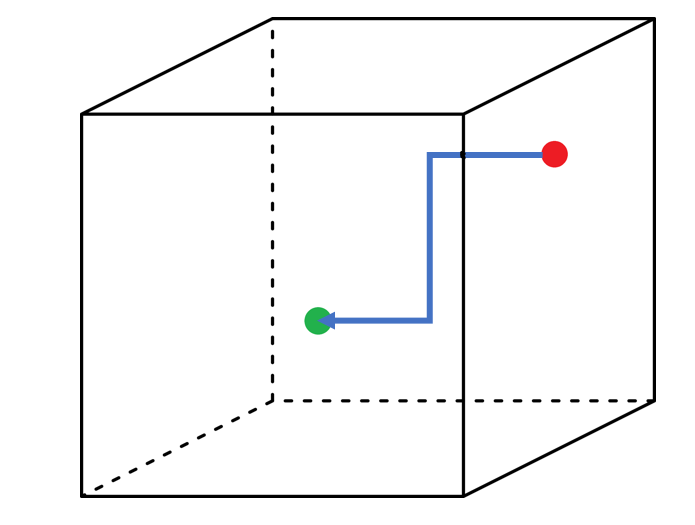
\includegraphics[width=0.6\linewidth]{cube.png}
  \caption{Схема работы алгоритма подбора параметров}
  \label{fig:cube}
\end{figure}

На схеме, изображённой на \picref{fig:cube}, куб изображает пространство конфигураций, красная точка~--- начальную точку, отвечающей начальной конфигурации процессора, зелёная точка~--- желаемую точку, в которой достигается максимальное (либо требуемое) IPC.

Рассмотрим пространство конфигураций более подробно. Обычно параметры микроархитектуры процессора могут принимать лишь дискретный набор значений, следовательно число точек в пространстве конфигураций конечно и может быть вычислено по правилу умножения~\cite[25]{окулов2014дискретная}:
\begin{equation}\label{eq:NG}
  N_G = \prod_{i = 1}^{n} \left|p_i\right|,
\end{equation}
где $p_i$~--- множество значений параметра с индексом $i$, $\left|p_i\right|$~--- его мощность (количество значений параметра с индексом $i$), при этом очевидно, что $\forall i \,\,\, x_i \in p_i$.

Пусть $\Delta t$~--- время однократного исполнения трассы на симуляторе, $N$~--- число точек конфигурационного пространства, в которых требуется исполнить трассу. Тогда полное время исполнения одной трассы на симуляторе в $N$ точках пространства конфигураций вычисляется по очевидной формуле:
\begin{equation}\label{eq:TN}
  T_N = N \cdot \Delta t.
\end{equation}

Используя формулы \formref{eq:NG} и \formref{eq:TN}, можно оценить время, требуемое для исполнения одной трассы во всех точках пространства конфигураций (метод полного перебора):
\begin{equation}\label{eq:bf_time}
  T_{G} = N_G \cdot \Delta t = \prod_{i = 1}^{n} \left|p_i\right| \cdot \Delta t.
\end{equation}

Решение методом полного перебора, очевидно, способно найти точку конфигурационного пространства с наибольшим IPC, однако из-за огромного числа параметров современного процессора, а также длительного времени симуляции на моделях производительности, время $T_G$ из \formref{eq:bf_time} становится значительно больше разумных сроков для решения данной задачи. В этой связи разрабатываются подходы, уменьшающие время работы симулятора для нахождения оптимальной конфигурации процессора. Исходя из формулы \formref{eq:TN}, можно разделить потенциальные методы решения задачи поиска оптимальной конфигурации микроархитектуры процессора на два класса:
\begin{itemize}
  \item решения, уменьшающие $\Delta t$~--- методы ускорения симуляции
  \item решения, уменьшающие $N$~--- методы ускорения непосредственно алгоритма подбора через уменьшение числа точек пространства конфигураций, в которых требуется запустить симулятор
\end{itemize}

Перейдём к рассмотрению существующих методов\,--\,представителей вышеперечисленных классов.

\section{Решения, уменьшающие время симуляции}

Данный класс решений фокусируется на ускорении работы симулятора. Методы данного класса предлагают использовать аппаратные решения~\cite{chiou2007fpga}, а также ряд оптимизаций на программном уровне~\cite{miller2010graphite,carlson2011sniper}.

Нетрудно заметить, что  с увеличением числа параметров и количества их значений число симуляций $N_G$ сильно растёт, и ускорение, получаемое методами данного класса, нивелируется, не оказывая заметного влияния на возрастание $T_G$.

\section{Решения, ускоряющие алгоритм подбора}

\subsection{CPI stack подходы}

В данных подходах используется метод CPI stack, в основе которого лежит идея о разложении среднего числа тактов, потраченных на одну исполненную инструкцию~--- CPI~\formref{eq:CPI} на независимые слагаемые. Обычно выделяют базовую (обязательную), а также некоторый набор компонент, отражающих такты, <<потерянные>> из-за таких событий как ошибки предсказания переходов, промахи в кэшах и буферах ассоциативной трансляции (англ.~TLB) и т.~д.~\cite{eyerman2006performance}:
\begin{align}\label{eq:CPIstack}
  \begin{split}
    \text{CPI} &= \dfrac{
      \text{обязательные такты} + \text{такты на кэш} + \text{такты на TLB} + \dots
      }{\text{число исполненных инструкций}}\\
      &= \frac{\text{обяз. такты}}{\text{число исп. инструкций}} + \frac{\text{такты кэш}}{\text{число исп. инструкций}} + \dots\\
      &= \text{CPI}_{\text{обяз}} + \text{CPI}_{\text{кэш}} + \text{CPI}_{\text{TLB}} + \dots
  \end{split}
\end{align}

При аккуратном подсчёте, CPI stack позволяет указать на узкие места в конфигурации процессора, сужая множество параметров\,--\,кандидатов на изменение. Например, в~\cite{lee2014rpstacks} рассматривается использование CPI stack полученного с помощью анализа критического пути в конвейере процессора. Такой подход позволяет более точно оценить причины потери циклов процессора, однако анализ критического пути является затратной (а также сложной в реализации) операцией, значительно увеличивающей время симуляции. Именно поэтому в~\cite{eyerman2017multi} предлагается вместо усложнения алгоритма вычисления CPI stack, вычислять сразу несколько CPI stack на разных стадиях конвейера процессора. Данное представление даёт более полную картину о событиях, влияющих на производительность процессора, а также диапазон ожидаемых улучшений производительности процессора в случае ликвидации конкретного события простоя.


\subsection{Подходы с использованием машинного обучения}


Исходя из теоретического описания задачи, представленного в разделе~\ref{sec:theor_base}, можно заключить, что рассматриваемая задача сводится к задаче оптимизации, для решения которой можно использовать методы машинного обучения.

Подходы с использованием машинного обучения~\cite{joseph2006construction,ipek2006efficiently,chen2014archranker} предлагают использовать модели, обученные на некотором относительно небольшом подмножестве пространства конфигураций, для предсказания IPC во всех остальных точках пространства.
Например, в~\cite{joseph2006construction} предлагается решать задачу подбора параметров как задачу линейной регрессии:
% \[
  \begin{multline}
    y = \beta_0 + \sum_{i = 1}^{m} \beta_i x_i + \sum_{i = 1}^{m}\sum_{j = i + 1}^{m}\beta_{i,j}x_ix_j \\  +\sum_{i = 1}^{m}\sum_{j = i + 1}^{m}\sum_{k = j + 1}^{m} \beta_{i,j,k} x_ix_jx_k
    \dots \\  +\beta_{1,2,\dots,m}x_1x_2\dots x_m,
  \end{multline}
% \]
где в качестве выходного параметра $y$ выступает CPI (дополнительно проводится исследование с целью выбрать функцию от IPC в качестве выходного параметра, которая обладает наименьшей ошибкой), а подбираемые коэффициенты $\beta$ играют роль важности соответствующего параметра. В работе также указывается, что для хорошей сходимости и высокой точности решения обычно достаточно не слишком большое множество параметров микроархитектуры процессора~--- достаточно лишь выделить некое подмножество.

В~\cite{ipek2006efficiently} применяется более сложный подход с использованием моделей нейронных сетей. В работе предлагается модель, которой достаточно обучится на 1\% от всего пространства конфигураций, для того чтобы выдавать высокоточные предсказания. Перед передачей параметров процессора нейронной сети, производится их нормировка в интервал $(0,1)$ c помощью min max scaling~\cite[114]{han2012data}, включая категориальные параметры (для них используется метод one-hot encoding~\cite{brownlee2017one}). Далее происходит тренировка некого набора нейронных сетей с применением перекрёстной валидации~\cite{stone1978cross}. Также стоит отметить, что каждая точка конфигурационного пространства из тренировочного набора подается сетям с частотой, пропорциональной CPI в этой точке.

В противовес предыдущему решению, в~\cite{chen2014archranker} описывается несколько иной подход с использованием машинного обучения, решая вместо классической задачи нахождения экстремального значения, задачу классификации. Данная задача состоит в том, чтобы выделить из двух предоставленных конфигураций микроархитектуры процессора <<лучшую>>. Такие попарные сравнения позволяют без дополнительных расходов на симуляцию увеличить размер тренировочного множества с $n$ до $\frac{n\cdot \left(n - 1 \right)}{2} = \mathcal{O}\left(n^2\right)$, что существенно улучшает точность предсказания.

В~\cite{dubach2010empirical} сообщается о двух недостатках, которыми обладают некоторые вышеописанные модели:
\begin{itemize}
  \item При смене тестовых наборов требуется заново собирать и обучать модель
  \item Для обучения существующих предсказателей обычно требуется большое число симуляций
\end{itemize}
Предлагаемая модель фокусируется на поведении самой микроархитектуры. В основе метода лежит идея о разложении нового пространства, представляющего новую программу на на линейную комбинацию пространств тестовых программ, где в роли метрики выступает производительность.
\begin{figure}[!ht]
  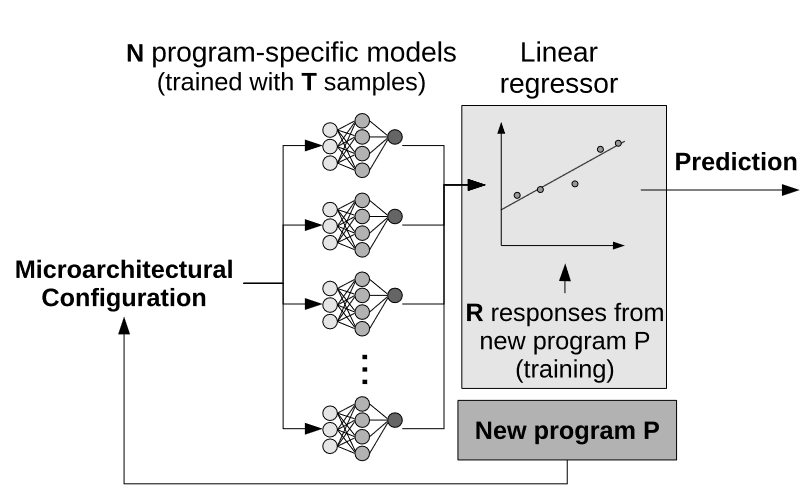
\includegraphics[width=\linewidth]{ML.png}
  \caption{Схема алгоритма~\cite{dubach2010empirical}}
  \label{fig:empirical}
\end{figure}
На \picref{fig:empirical} изображена схема предлагаемого решения. Решение работает следующим образом. Сначала происходит обучение $N$ моделей, каждая на своём приложении, далее при для предсказания  поведения новой программы, собирается результат малого числа $R$ симуляций новой программы, а также результаты предсказаний моделей с этих симуляций, после чего используется метод линейной регрессии в следующем виде:
\[
  \lvec{y} = \beta_0 + \sum_{i = 1}^{m} \beta_i \cdot \lvec{X}_i,
\]
где $\lvec{X}_j$~--- вектор из $R$ ответов от модели $j$, $\lvec{y}$~--- вектор, состоящий из ответов новой программы на $R$ симуляциях. Таким образом, для получения предсказания для новой программы на очередной точке конфигурационного пространства, достаточно подать $R$ новых точек пространства на обученные предсказатели (модели), получая тем самым нужные $R$ ответов.

Перечисленные методы позволяют значительно сократить число симуляций $N$.

\section{Анализ решений}

В существующих работах, как правило, рассматривается варьирование параметров высокого порядка\footnote{Параметры, небольшое изменение которых приводит к значительному изменению производительности}, такие как размер кэша, алгоритм предсказания условных переходов и т.~п. В то время как наибольшую сложность на практике представляет варьирование параметров низкого порядка (дополнительный бит в алгоритме предсказания, дополнительный бит тэга).

С одной стороны, исходя из определения, изменение одного параметра микроархитектуры низкого порядка не может привести к такому значительному изменению производительности процессора, как при изменении одного параметра микроархитектуры высокого порядка. С другой стороны, при одновременном изменении нескольких параметров микроархитектуры низкого порядка, можно добиться существенного прироста производительности процессора.

Существующие решения не позволяют эффективно находить оптимальные конфигурации микроархитектуры процессора при рассмотрении большого числа параметров низкого порядка:
\begin{itemize}
  \item Подходы основанные на RpStacks имеют высокую сложность реализации, в силу того, что стандартные данные о задержках, предоставляемые разработчиками симуляторов, не покрывают эффективно параметры микроархитектуры низкого порядка.
  \item Эмпирические модели машинного обучения, которые предлагается использовать для предсказания производительности процессора, из-за нетривиального характера взаимного влияния параметров низкого порядка требуют намного больше данных для обучения, что выражается в большем числе запуска симулятора, отрицательно сказываясь на времени работы
\end{itemize}


\chapter{Методология}

В данной главе приводится описание предлагаемого решения. Сначала описывается непосредственно алгоритм подбора параметров микроархитектуры процессора, логика его работы. Далее приводится обзор среды моделирования, на которой производились запуски алгоритма подбора. В конце главы рассматривается инфраструктура, позволяющая упростить работу среды моделирования со статистикой.
\section{Описание алгоритма подбора}

Предлагаемый алгоритм подбора оптимальной конфигурации основан на отображении набора статистических данных, получаемых в результате симуляции, на параметры конфигурации процессора. В рассматриваемом алгоритме используются статистические данные, которые, как правило, появляются в больших промышленных и академических симуляторах производительности естественным образом в ходе работы над улучшениями микроархитектуры; либо несложным образом выражаются через стандартные статистические данные.

Каждому статистическому значению сопоставляется определённое множество параметров (непосредственно влияющих на данное статистическое значение) процессора, которым, в свою очередь, сопоставляются наборы возможных (варьируемых) значений. Упомянутые наборы определяют \textbf{пространство конфигураций}.

На каждой итерации алгоритма выполняются следующие действия:
% \begin{algorithm}
%   \caption{Описание алгоритма подбора}
%   \begin{algorithmic}
%     \State $предIPC \gets -1$
%     \Statex
%     \While{Есть доступные модификации}
%     \State $ЗапуститьСимулятор()$
%     \State $стаистика,\,IPC \gets СобратьСтатистику()$
%     \If{$предIPC \neq -1$}
%       \State $разница \gets IPC - предIPC$
%       \If{$разница < 0$}
%         \State $ОткатитьИзменение()$
%         \State $ИсключитьСтатистику из ()$
%       \EndIf
%     \EndIf
%     \EndWhile
%     \If{$i\geq 5$}
%     \State $i \gets i-1$
%     \Else
%     \If{$i\leq 3$}
%     \State $i \gets i+2$
%     \EndIf
%     \EndIf
%   \end{algorithmic}
% \end{algorithm}

\begin{enumerate}
  \item Запустить симулятор, собрать и усреднить статистические данные по трассам исполнения
  \item Вычислить  изменение IPC по сравнению с предыдущей итерацией
  \item Если изменение отрицательное, произвести откат последнего изменения параметра и исключить зависимую статистику из списка кандидатов до тех пор, пока переходом к другой точке пространства конфигураций не будет получено положительное изменение IPC (\picref{fig:rollback})
  \item Выбрать из списка кандидатов имеющее наибольшее относительное отклонение от порогового\footnote{Подбираются на основе предварительных инициализирующих запусков} статистическое значение
  \item Запросить изменение параметра конфигурации, от которого зависит выбранное статистическое значение
\end{enumerate}

\begin{figure}[!htbp]
  \centering
  \scalebox{1}{
  \begin{tikzpicture}
    \draw[step=1.5cm,gray,thin] (-1.5,-1.5) grid (3,3);
    \draw[black, thick] (0, 0) circle (4 pt);
    \draw[-Latex, ultra thick, midway, red] (0,0) -- node[right, black] {1} ++ (0,1.5);
    \draw[-Latex, ultra thick, dashed, midway] (-0.2,1.5) -- node[left] {2} ++ (0,-1.5);
    \draw[-Latex, ultra thick, midway, Green] (0,0) -- node[below, black] {3} ++ (1.5,0);
    \draw[thick,->, midway](-1.5,-1.5) -- node[below]{Параметр A} ++ (4.5,0);
    \draw[thick,->, midway](-1.5,-1.5) -- node[rotate=90,above]{Параметр B} ++ (0,4.5);
  \end{tikzpicture}
  }
  \caption{Принцип работы отката изменения}
  \label{fig:rollback}
\end{figure}

Описанный выше порядок действий повторяется до тех пор, пока не выполнится одно из условий:
\begin{itemize}
  \item Достижение требуемого улучшения производительности (если было задано)
  \item Исчерпание возможных направлений модификаций
  \item Превышение лимита числа итераций (если был задан)
\end{itemize}

\begin{figure}[!htbp]
  \centering
  \scalebox{0.862}{
    \begin{tikzpicture} [
    scale=1,
    -Latex,auto,node distance =1 cm and .4 cm, thick,% node distance is the distance between one node to other, where 1.5cm is the length of the edge between the nodes
  ]
  % values

  \node[state, fill=Cyan] (v1) {Значения};
  \node[state, fill=Cyan] (v2) [below of=v1] {Значения};
  \node[state, fill=Cyan] (v3) [below of=v2] {Значения};
  \node[state, fill=Cyan] (v4) [below of=v3] {Значения};
  \node[state, fill=Cyan] (v5) [below of=v4] {Значения};
  \node[state, fill=Cyan] (v6) [below=.7cm of v5] {Значения};
  \node[state, fill=Cyan] (v7) [below=.7cm of v6] {Значения};

  % params

  \node[state, fill=Apricot] (p1) [right = of v1] {Параметр 1};
  \node[state, fill=Apricot] (p2) [right = of v2] {Параметр 2};
  \node[state, fill=Apricot] (p3) [right = of v3] {Параметр 3};
  \node[state, fill=Apricot] (p4) [right = of v4] {Параметр 4};
  \node[state, fill=Apricot] (p5) [right = of v5] {Параметр 5};
  \node[state, fill=Apricot] (p6) [right = of v6] {Параметр k};
  \node[state, fill=Apricot] (p7) [right = of v7] {Параметр n};

  \path (p5) -- node[auto=false]{\ldots} (p6);
  \path (p6) -- node[auto=false]{\ldots} (p7);

  % params -> values
  \draw[->] (p1) -- (v1);
  \draw[->] (p2) -- (v2);
  \draw[->] (p3) -- (v3);
  \draw[->] (p4) -- (v4);
  \draw[->] (p5) -- (v5);
  \draw[->] (p6) -- (v6);
  \draw[->] (p7) -- (v7);

  % stat vals

  \node[state, rectangle, fill=LimeGreen] (s2) [right = of p4] {Статистическое \\значение 2};
  \node[state, rectangle, fill=LimeGreen] (s1) [right = of p1, above =0cm of s2] {Статистическое \\значение 1};
  \node[state, rectangle, text=white] (sdots) [below=0cm of s2] {Статистическое \\значение 3};
  \node[state, rectangle, fill=LimeGreen] (s3) [right = of p6, below =0cm of sdots] {Статистическое \\значение M};

  \path (s2) -- node[auto=false]{\ldots} (s3);
  \draw [-,OrangeRed,decorate,thick,decoration={brace,amplitude=15pt, mirror},yshift=5cm,xshift=0pt]
  (s3.south west) -- (s3.south east) node [black,midway,yshift=-1cm]{\footnotesize Вектор статистик};


  % s to p

  \draw[->, bend right] (s1.north) to (p1.east);
  \draw[->] (s1.north) -- (p2.east);

  \draw[->, bend right] (s2.west) to (p3.east);
  \draw[->] (s2.west) -- (p4.east);
  \draw[->, bend left] (s2.west) to (p5.east);

  \draw[->] (s3.west) -- (p6.east);
  \draw[->] (s3.west) -- (p7.east);

  % big nodes

  \node[state, fill=NavyBlue!60] (choice) [right = of s2] {Выбор наиболее \\отклонившегося \\значения};

  \node[state, fill=cyan!60] (thres) [below = of choice] {Пороговые \\значения};

  \draw[->] (thres) -- (choice);

  \draw[->] (s1.east) -- (choice);
  \draw[->] (s2.east) -- (choice.west);
  \draw[->] (s3.east) -- (choice);

  \node[state, fill=lime!50] (fin) [above = of choice] {Изменение зависимых \\параметров выбранного \\значения
  };

  \draw[->] (choice) -- (fin);
\end{tikzpicture}

  }
  \caption{Схема работы алгоритма}
\end{figure}



\section{Обзор среды моделирования}

Для тестирования предложенного алгоритма требовалось разработать среду моделирования, которая бы позволяла взаимодействовать с симулятором (например, для изменения параметров), а также производила сбор статистики полученной с трасс исполнения.

В силу большого разнообразия симуляторов, ориентированных под различные нужды, и как следствие значительных отличий в организации работы с ними, была поставлена задача сделать среду моделирования \textbf{симуляторонезависимой}~--- способной выступать в роли связующего звена между конкретным симулятором и алгоритмом, не вмешиваясь в работу последнего. Кроме того, из-за большого числа трасс исполнения в тестовых наборах приложений, было необходимо, чтобы среда моделирования поддерживала запуск нескольких трасс исполнения в параллельных потоках для уменьшения время работы алгоритма и лучшей утилизации вычислительных ресурсов кластерных систем, на которых и предполагается запуск реализованного алгоритма.

Схема работы реализованной среды моделирования представлена на \picref{fig:framework}.

Далее представлено описание элементов схемы.

\begin{itemize}
  \item \textbf{Обобщённый интерфейс} позволяет абстрагироваться от конкретного симулятора, обеспечивая взаимодействие с ним в обобщённом виде. Для добавления поддержки нового симулятора достаточно лишь описать ключевые моменты в работе с ним (процесс запуска, сбор статистики, изменение параметров), при этом не требуется вносить изменения в остальную (<<алгоритмическую>>) часть среды моделирования.
  \item \textbf{Алгоритм подбора} через обобщённый интерфейс получает от симулятора статистические данные запуска трасс исполнения. Далее происходит усреднение статистических данных, а также прироста IPC по трассам исполнения. Для того, чтобы получить осмысленное среднее значение прироста IPC, производится предварительная нормировка каждого значения IPC на значение на начальной итерации (под номером $0$) по формуле
  \[
    \text{IPC}_{ij}^{norm} = \dfrac{\text{IPC}_{ij}}{\text{IPC}_{0j}},
  \]
  где $i$~--- номер итерации, $j$~--- номер трассы исполнения. Тогда относительный прирост IPC на итерации $i$ для трассы $j$ может быть вычислен как
  \[
    \Delta \text{IPC}_{ij} = \text{IPC}_{ij}^{norm} - 1.
  \]
  В итоге среднее значение относительного прироста IPC вычисляется как
  \[
    \left\langle \Delta\text{IPC}_{i}\right\rangle =
    \sqrt[M]{\prod_{j = 1}^{M} \Delta \text{IPC}_{ij}}
  \]
  При этом среднее значение статистического значения  вычисляется по формуле
  \[
    \left\langle \text{Stat}_{i} \right\rangle =
    \dfrac{\displaystyle\sum_{j = 1}^{M} \text{Stat}_{ij}}{M},
  \]
  где $\text{Stat}_{ij}$ (по аналогии с IPC) есть статистическое значение с именем Stat, полученное с трассы исполнения с номером $j$ на $i$-ой итерации.

  На основании анализа статистики, через обобщённый интерфейс осуществляется запрос изменения выбранного зависимого параметра.
  \item \textbf{Кластер} (либо иная среда с возможностью параллельного исполнения) осуществляет параллельный запуск трасс исполнения на симуляторе.
\end{itemize}

\begin{figure}[ht!]
  \centering
  \scalebox{0.932}{
    \begin{tikzpicture} [
    scale=1,
    -Latex,auto,node distance =1 cm and .4 cm, thick,% node distance is the distance between one node to other, where 1.5cm is the length of the edge between the nodes
  ]
  % simulators

  \node[state, fill=Apricot] (s1) {Симулятор 1};
  \node[state, fill=Apricot] (s2) [below=.4cm of s1] {Симулятор 2};
  \node[state, fill=Apricot] (s3) [below=of s2] {Симулятор n};

  % interface
  \node[state] (int) [right=of s2, fill=LimeGreen] {Обобщённый \\интерфейс};

  \draw[->] (s1) -- (int);
  \draw[->] (s2) -- (int);
  \draw[->] (s3) -- (int);

  \path (s2) -- node[auto=false]{\ldots} (s3);


  \node[state] (dse) [right=of int, fill=LimeGreen] {Алгоритм \\подбора};
  \draw[->] (int) -- (dse);

  \node[state] (req) [above=of int, fill=cyan!50] {Запрос \\изменений};
  \draw[->] (dse) -- (req);
  \draw[->] (req) -- (int);

  \node[state] (change) [below=of int, fill=cyan!50] {Изменение \\параметров};

  \draw[->, thick, dashed, in=90] (s2.west) -- (s1.west);
  \draw[->, thick, dashed] (s3.west) -- (s2.west);
  \draw[->, thick, dashed] (change) -| (s3.west);

  \draw[->] (int) -- (change);

  \node[state] (traces) [below=of dse, fill=NavyBlue!60] {Трассы \\исполнения};
  \draw[->] (traces) -- (dse);

  \node[state] (stat) [above=of dse, fill=lime!50] {Статистика};
  \draw[->] (stat) -- (dse);

  % cluster
  \node[state, fill=NavyBlue!60] (t3) [right=.7cm of dse] {Трасса 3};
  \node[state, fill=NavyBlue!60] (t2) [above=.1cm of t3]  {Трасса 2};
  \node[state, fill=NavyBlue!60] (t4) [below=1.3cm of t3]  {Трасса M};
  \node[state, fill=NavyBlue!60] (t1) [above=.1cm of t2]  {Трасса 1};

  \path (t3) -- node[auto=false]{\ldots} (t4);

  \begin{scope}[on background layer]
    \node[draw, thick, fit=(t1)(t2)(t3)(t4), fill=Apricot] (cluster) [right=of dse] {};
  \end{scope}
  \draw[->, bend right] ([xshift=-1.1cm]cluster.north) to (stat.north);
  \node at (cluster.north) [above=.1cm of t1] {Кластер};

  \draw[->] (dse) -- (t3-|cluster.west);
\end{tikzpicture}

  }
  \caption{Схема работы среды моделирования}
  \label{fig:framework}
\end{figure}

В среде моделирования реализована поддержка двух симуляторов производительности: gem5~\cite{binkert2011gem5} и ChampSim~\cite{gober2022championship}.

Для валидации работы алгоритма был добавлен режим полного перебора, в котором осуществляется проход по всем точкам конфигурационного пространства с запуском на них симулятора для нахождения максимально возможного IPC. По этой причине при выборе параметров для варьирования требовалось ограничиться небольшим числом параметров, чтобы алгоритм полного перебора успел просчитать все точки конфигурационного пространства за разумное время.

\section{Работа со статистикой в обобщённом виде}

В силу того, что формат хранения статистических данных сильно отличается от симулятора к симулятору (начиная с разных форматов файлов статистики и заканчивая различными названиями статистических данных и параметров), требовалось спроектировать инфраструктуру, которая бы обеспечила единообразный подход к анализу статистики с точки зрения алгоритма подбора.

\begin{listing}[!htbp]
  \centering
  \inputminted{js}{listings/mappings.json}
  \caption{Пример файла отображений}
  \label{lst:mappings}
\end{listing}

Каждый симулятор сопровождается файлом в формате JSON~\cite{bray2014javascript}, который называется \textbf{файлом отображений} (англ.~mappings file).


В листинге \ref{lst:mappings} представлен пример такого файла. В нём можно заметить две основные секции: определение множества варьируемых параметров с их отображением на статистические данные (по ключу \mintinline{js}{"statistics->parameters"}), а также соотнесение названий статистических данных симулятора с их обобщёнными аналогами (по ключу с именем \mintinline{js}{"statistics->generalized"}). Кроме того, в листинге \ref{lst:mappings} представлены все поддержанные варианты задания значений для параметров: строка, целое число, либо список целых чисел.

В ходе работы алгоритма, статистические значения (в обобщённом виде) сравниваются с пороговыми значениями, полученными в результате инициализирующих запусков симулятора. Они определены в \textbf{файле пороговых значений} (англ.~thresholds file) в формате JSON~\cite{bray2014javascript}. Пример такого файла представлен в листинге \ref{lst:thres}.

\begin{listing}[!ht]
  \centering
  \inputminted{js}{listings/thres.json}
  \caption{Пример файла пороговых значений}
  \label{lst:thres}
\end{listing}


Описанная выше инфраструктура позволяет алгоритму подбора оперировать исключительно обобщённой статистикой.


\chapter{Результаты}


В качестве симулятора производительности использовалась модель суперскалярного процессора с внеочередным исполнением команд архитектуры ARM~\cite{seal2001arm}, основанная на симуляторе gem5~\cite{binkert2011gem5}. В ходе работы в симулятор был добавлен подсчёт статистики для работы алгоритма подбора.

Запуски осуществлялись с помощью реализованной среды моделирования в режиме параллельного исполнения на наборе тестовых 3D\,--\,приложений.

Перед запуском была проведена предварительная обработка данных, с целью выделения групп (кластеров) приложений со схожими <<горячими>>\footnote{Значения, имеющие наибольшее относительное отклонение от своих пороговых значений} статистическими значениями. Для улучшения результатов кластеризации, была проведена нормализация данных. В результате предварительной обработки данных, было выделено два кластера, по которым в дальнейшем и производилось усреднение статистических значений.

Для оценки результата работы предложенного алгоритма, были проведены запуски в двух режимах:
\begin{itemize}
  \item Обычный режим (поиск оптимальной конфигурации с помощью предложенного алгоритма)
  \item Режим полного перебора~--- обход всех точек пространства конфигураций с нахождением максимально возможного IPC
\end{itemize}

В результате вышеописанных запусков, был получен прирост производительности, в среднем отклоняющийся на 3.2\% от оптимального прироста производительности (полученного методом полного перебора). Среднее улучшение производительности составило 2.22\%, причём для достижения этого результата потребовалось в среднем обойти всего 14\% от общего числа точек пространства конфигураций.

Полученный результат позволяет сделать вывод о том, что предложенный алгоритм способен успешно подбирать оптимальную конфигурацию процессора с производительностью, незначительно отличающейся от максимально возможной на заданном конфигурационном пространстве. Кроме того, алгоритму требуется значительно меньшее число точек конфигурационного пространства для обнаружения точки с оптимальной производительностью.


\chapter{Заключение}

В работе был предложен алгоритм оптимального подбора параметров, основанный на идее отображения статистических данных, полученных с симулятора, на параметры процессора.

Для использования и тестирования алгоритма была разработана среда моделирования с поддержкой обобщенного интерфейса работы с симуляторами. Данная среда моделирования также обладает возможностью запуска трасс исполнения в параллельном режиме.

С помощью тестовых запусков было выяснено, что предложенный алгоритм позволяет находить оптимальную конфигурацию микроархитектуры процессора через варьирование параметров низкого порядка.

В результате работы алгоритма на тестовом наборе приложений было получено среднее увеличение производительности на 2.22\%, при этом отклонение этого значения от максимально возможного прироста производительности, полученного методом полного перебора, составило 3.2\%.



\backmatter{}
\printbib{}

% \chapter{Благодарности}
% Благодарности идут тут.

\end{document}
